\section{实验结果}

\subsection{英德翻译结果}

\begin{table}[!htbp]
    \bicaption{基于RNN的神经翻译模型在Multi30K数据集英译德翻译方向的实验结果}{Experiment results of RNN-based NMT on the Multi30K En-De translation pair.}
    \label{tab:3_rnn_ende}
    \centering
    \footnotesize% fontsize
    \setlength{\tabcolsep}{4pt}% column separation
    \renewcommand{\arraystretch}{1.2}%row space 
    \begin{tabular}{cccccccc}
        \hline
        \multicolumn{2}{c}{\multirow{2}{*}{基于RNN}} & \multicolumn{2}{c}{Test2016} & \multicolumn{2}{c}{Test2017} & \multicolumn{2}{c}{MSCOCO} \\ \cline{3-8}
                  & & BLEU        & METEOR      & BLEU         & METEOR        & BLEU         & METEOR   \\ %\hline
    \hline
    \multicolumn{2}{c}{NMT}                                                 & 35.9  & 54.9   & 28.8   & 49.5   & 25.9   & 45.7  \\ %\hline
    \hline
    \multicolumn{2}{c}{pRCNNs \cite{35_huang-etal-2016-attention}}             & 36.5   & 54.1   & -           & -           & -           & -           \\
    \multicolumn{2}{c}{DATT \cite{36_calixto-etal-2017-doubly}}                & 36.5        & 55.0        & -           & -           & -           & -           \\
    \multicolumn{2}{c}{Imagination \cite{37_elliott-kadar-2017-imagination}}   & 36.8   & 55.8   & -           & -           & -           & -           \\
    \multicolumn{2}{c}{$ \mathrm{VMMT_C} $ \cite{38_calixto-etal-2019-latent}} & 37.5   & 55.7   & 26.1   & 45.4   & 21.8   & 41.2   \\
    \multicolumn{2}{c}{$ \mathrm{VMMT_F} $ \cite{38_calixto-etal-2019-latent}} & 37.7   & 56.0   & 30.0   & 49.9   & 25.5   & 44.8   \\ \hline%\hline
                      
    \multirow{3}*{词级} & 
       独享-源   & 37.8           & 56.1           & 30.1           & \textbf{50.3}  & \textbf{27.0}  & \textbf{46.4}  \\
     & 共享-源   & \textbf{38.0}  & 56.2           & 30.3           & 50.1           & 26.1           & 45.6  \\
     & 共享-目    & 36.3           & 55.0           & 28.4           & 48.6           & 25.3           & 44.3  \\ %\hline
    \hline
    \multirow{3}*{短语级} & 
        独享-源  & \textbf{38.0}  & \textbf{56.5}  & 30.2           & \textbf{50.3}  & 26.8           & 46.1  \\
     &  共享-源  & 37.8           & 56.1           & \textbf{30.5}  & 50.1           & 26.0           & 45.5  \\
     &  共享-目  & 36.8           & 55.0           & 29.4           & 49.0           & 26.3           & 45.3  \\ 
        \hline
    \end{tabular}
\end{table}
如\ref{sec:3_entity_replacement}和\ref{sec:3_parameter_sharing}节所述,本章共设置了两种实体替换规则:短语级和词级,以及三种模型参数共享策略:独享解码器重构源语言、共享解码器重构源语言以及共享解码器重构目标语言,并分别以“独享-源”、“共享-源”和“共享-目”作为简化表示,对以上实验配置进行组合后共得到6种模型设置方案。另外,本章还针对以上设置在基于RNN和基于Transformer的机器翻译模型上都进行了实验,并在BLEU\pcite{papineni2002bleu}和Meteor\pcite{denkowski2014meteor}两个指标上进行比较。

{\sffamily 基于RNN的模型实验结果:}表\ref{tab:3_rnn_ende}展示了采用基于RNN的神经机器翻译模型在英译德翻译对上的实验结果,其中加粗项表示同列中最好的实验结果。本章与5个融合图片信息的神经机器翻译方法进行了对比,其中pRCNNs和DATT需要在测试过程中为模型输入图片,其它模型包括本章所设计的翻译模型在测试阶段不需要输入图片。该实验结果展示了本章所提方法在纯文本翻译的基础上得到了显著的提升,表明了CTR-NMT在基于RNN的模型上的有效性。该实验结果同样显示出了6种实验方案的优缺点。对于重构到源语言句子,实验结果中没有表现出采用共享解码器或独享解码器两种配置之间的明显差距,同样在采用词级替换规则或是短语级替换规则中的差别也不大。对于重构到目标语言句子,可以观察到其实验结果明显的低于重构到源语言的方案。以上信息表明,为重构任务设置的语言方向是影响本章所提方法实验效果的最大因素。


\begin{table}[!htbp]
    \bicaption{基于Transformer的神经翻译模型在Multi30K数据集上的实验结果}{Experiment results of Transformer-based NMT on the Multi30K dataset.}
    \label{tab:3_transformer_ende}
    \centering
    \footnotesize% fontsize
    \setlength{\tabcolsep}{4pt}% column separation
    \renewcommand{\arraystretch}{1.2}%row space 
    \begin{tabular}{lccccccc}
        \hline
        \multicolumn{2}{c}{\multirow{2}{*}{基于Transformer}} & \multicolumn{2}{c}{Test2016} & \multicolumn{2}{c}{Test2017} & \multicolumn{2}{c}{MSCOCO} \\ \cline{3-8}
                  & & BLEU        & Meteor      & BLEU         & Meteor        & BLEU         & Meteor   \\ %\hline
    \hline
    \multicolumn{2}{l}{~~~~Transformer}                                     & 38.5       & 57.5      & 31.0   & 51.9   & 27.5   & 47.4     \\\hline
    \multicolumn{2}{l}{~~~~DelMMT \pcite{ive2019distilling}}          & 38.0            & 55.6           & -           & -           & -           & -             \\
    \multicolumn{2}{l}{~~~~MMT-TF \pcite{yao2020multimodal}}           & 38.7            & 55.7           & -           & -           & -           & -             \\
    \multicolumn{2}{l}{~~~~GAMMT \pcite{liu2021gumbel}}  & 39.2            & \textbf{57.8}  & 31.4        & 51.2        & 26.9        & 46.0          \\
    \multicolumn{2}{l}{~~~~GMMT \pcite{yin2020novel}}                 & \textbf{39.8}   & 57.6           & 32.2        & 51.9        & 28.7        & \textbf{47.6} \\ \hline%\hline
    \multicolumn{8}{c}{CTR-NMT}\\\hline
    \multirow{3}*{~~词级} & 
       独享-源   & 39.7       & 57.5             & \textbf{32.9}    & 51.7             & \textbf{29.1}    & 47.5   \\
     & 共享-源   & 39.4       & \textbf{57.8}    & 32.4             & \textbf{52.1}    & 28.3             & 47.5   \\
     & 共享-目   & 38.7       & 56.2             & 31.0             & 49.6             & 26.5             & 44.9     \\ %\hline
    \hline
    \multirow{3}*{~~短语级} & 
        独享-源  & 39.3       & 57.4             & 32.7             & 51.8             & 28.7             & 47.5   \\
     &  共享-源  & 39.0       & 57.3             & 32.4             & 51.6             & 28.3             & 47.2   \\
     &  共享-目  & 38.5       & 56.2             & 30.5             & 49.7             & 26.8             & 45.6   \\
        \hline
    \end{tabular}
\end{table}
{\sffamily 基于Transformer的模型实验结果:}表\ref{tab:3_transformer_ende}展示了采用基于Transformer的神经机器翻译模型在英译德翻译对上的实验结果,其中加粗项表示同列中最好的实验结果。5个对比模型中,仅Transformer为纯文本神经机器翻译方法,其它4个模型均需要在测试阶段输入图片。而本章所提方法仅需要在训练阶段输入图片,在测试阶段并不需要。从模型结果的比较中可以观察到,本章所提方法能够有效地提升纯文本神经翻译模型的翻译准确率,在测试阶段没有输入图片的劣势情况下,CTR-NMT依旧与其它方法是可比的。另外,在基于6种模型设置方案的结果比较中可以观察到与基于RNN的模型有相似的现象,即重构的语言方向是影响方法性能的主要因素。该实验结果中还可以发现,词级替换规则的实验结果相比于短语级有小幅度的优势。


% Table generated by Excel2LaTeX from sheet 'flickr'
\begin{table}[!htbp]
    \bicaption{基于Flickr30K Entities标注实体的实验结果}{Experiment results on the annotated entities provided by Flickr30K entities}
    \label{tab:3_flickr30k_entities}
    \centering
    \footnotesize% fontsize
    \setlength{\tabcolsep}{4pt}% column separation
    \renewcommand{\arraystretch}{1.2}%row space 
    \begin{tabular}{clcccccccc}
    \hline
    \multicolumn{2}{c}{\multirow{2}{*}{模型}} & \multicolumn{4}{c}{基于RNN} & \multicolumn{4}{c}{基于Transformer} \\ \cline{3-10}
    & & \multicolumn{2}{c}{BLEU} & \multicolumn{2}{c}{METEOR} & \multicolumn{2}{c}{BLEU} & \multicolumn{2}{c}{METEOR} \\\hline

    \multirow{3}*{词级} & 
       独享-源   & \textbf{38.0}  & {$\uparrow$ 0.2}  & 56.1  & - 0.0           &  \textbf{39.9}  & {$\uparrow$ 0.2}  & \textbf{58.0}  & {$\uparrow$ 0.3}\\
     & 共享-源   & 38.0  & - 0.0                                    & 55.9  & {$\downarrow$ 0.3}           &  \textbf{39.5}  & {$\uparrow$ 0.1}  & 57.2   & {$\downarrow$ 0.6}        \\
     & 共享-目    & \textbf{36.7}  & {$\uparrow$ 0.4}  & \textbf{55.5}  & {$\uparrow$ 0.5}  &  38.0  & {$\downarrow$ 0.7}           & \textbf{56.9}  & {$\uparrow$ 0.7}\\ \hline
    \multirow{3}*{短语级} & 
       独享-源   & \textbf{38.1}  & {$\uparrow$ 0.1}  & \textbf{56.6}  & {$\uparrow$ 0.1}  &  \textbf{39.4}  & {$\uparrow$ 0.1}  & 57.3   & {$\downarrow$ 0.1}        \\
     & 共享-源   & 37.8  & - 0.0                                    & \textbf{56.2}  & {$\uparrow$ 0.1}  &  \textbf{39.3}  & {$\uparrow$ 0.3}  & 57.1   & {$\downarrow$ 0.2}        \\
     & 共享-目    & \textbf{36.9}  & {$\uparrow$ 0.1}  & \textbf{55.3}  & {$\uparrow$ 0.3}  &  \textbf{38.8}  & {$\uparrow$ 0.3}  & \textbf{56.6}  & {$\uparrow$ 0.4}\\ 
    \hline
    \end{tabular}%
\end{table}%
{\sffamily 基于标注实体的实验结果:}Flickr30K Entities数据集为Multi30K数据集标注了句子中名词短语与图片中视觉目标的对应关系。因此,为了将这些标注数据应用到本章的方法中,仅需要利用词性标注工具识别出这些短语中的名词。表\ref{tab:3_flickr30k_entities}为应用Flickr30K Entities在基于RNN和基于Transformer的模型上的实验结果。加粗项表示相比于表\ref{tab:3_rnn_ende}和表\ref{tab:3_transformer_ende}中相同模型配置下有翻译准确率提升的实验结果。可以观察到,在应用了标注数据后,多数模型都得到了少许翻译准确率的提升。此外还可以观察到,“独享-源”的实验结果普遍要略好于“共享-源”,即重构任务和翻译任务采用各自单独的解码器时效果更佳。

综合以上结果,词级替换规则略优于短语级,应用单独的解码器略优于共享解码器,重构的语言方向对方法有效性的影响最大,重构源语言句子带来的翻译准确率提升最多。

\subsection{对抗评估与消融实验}
\label{sec:3_adversarial_ablation}
% Table generated by Excel2LaTeX from sheet 'ablation'
\begin{table}[!htbp]
    \bicaption{对抗评估与消融实验}{Adversarial evaluation and ablation study}
    \label{tab:3_adversarial_ablation}
    \centering
    \footnotesize% fontsize
    \setlength{\tabcolsep}{4pt}% column separation
    \renewcommand{\arraystretch}{1.2}%row space 
    \begin{tabular}{llcccc}
    \hline
    \multicolumn{2}{c}{\multirow{2}{*}{基于RNN}} & \multicolumn{4}{c}{BLEU} \\ \cline{3-6}
     &        & 原图片          & 随机图片           & 随机单词            & 掩码 \\
    \hline
    \multirow{3}*{~~词级} & 
       独享-源 & \textbf{37.8}  & 37.4              & 37.1             & \underline{36.8} \\%              & 37.5 \\ 
     & 共享-源 & \textbf{38.0}  & 37.8              & \underline{37.6} & \underline{37.6} \\%              & 38.2 \\
     & 共享-目 & \textbf{36.3}  & \textbf{36.3}     & \underline{35.0} & 35.6 \\\hline%              & 37.4 \\ \hline
    \multirow{3}*{~~短语级} & 
       独享-源 & \textbf{38.0}  & 37.2              & 37.3             & \underline{36.9} \\%              & 37.2 \\
     & 共享-源 & \textbf{37.8}  & \underline{37.5}  & 37.6             & 37.6 \\%              & 38.2 \\
     & 共享-目 & \textbf{36.8}  & 36.2              & 35.9             & \underline{35.3} \\%              & 37.3 \\ 
    \hline
    \end{tabular}%
\end{table}%

\tcite{elliott2018adversarial}指出,存在部分融合图片信息的神经机器翻译方法所获得的翻译准确率提升与输入的视觉信息相关性不大。在对这部分模型的输入图像进行随机替换后,模型翻译准确率没有表现出显著的变化。因此,检验视觉信息是否在翻译模型中起了作用对于本章所提方法是一个必要的过程。可根据本章所提方法的结构,假设方法所带来的增益来源于视觉目标中的视觉信息,多任务学习策略,以及模型的抗噪声能力。为此,设计了以下实验来验证方法的有效性:

(1){\sffamily 噪声输入:}在该方案中,本章应用两种噪声输入方法:随机图片和随机单词。随机图片就是在数据集中随机选取图片,从而输入错误的视觉目标。随机单词是将原本替换为视觉目标的位置替换为在词表中随机选择的词。

(2){\sffamily 掩码输入:}在该方案中,输入序列中视觉目标的位置替换为一个特殊的单词“<mask>”,此时的重构模型类似于一个掩码语言模型(masked language model),区别在于重构模型采用了序列解码的方式。

将该对抗评估方案应用于基于RNN的模型上,得到结果如表\ref{tab:3_adversarial_ablation}所示,加粗项代表同一配置的模型中的性能最佳,下划线项代表最差。从表\ref{tab:3_adversarial_ablation}可以观察到,输入为原图像的模型均取得了最佳的性能,同时两组对抗实验均表现出较差的结果。采用掩码输入的方式整体效果最差,说明多任务的方式带来的增益效果并不是主要因素。该实验结果表明本章所提方法确实能够捕捉到视觉信息,从而为翻译准确率带来提升。

\subsection{重构模型的对抗评估与消融实验}
\label{sec:3_adversarial_ablation_rec}

% Table generated by Excel2LaTeX from sheet 'ablation'
\begin{table}[!htbp]
    \bicaption{重构模型的对抗评估与消融实验结果}{Results of adversarial evaluation and ablation study for reconstruction model}
    \label{tab:3_adversarial_ablation_rec}
    \centering
    \footnotesize% fontsize
    \setlength{\tabcolsep}{4pt}% column separation
    \renewcommand{\arraystretch}{1.2}%row space 
    \begin{tabular}{llcccc}
    \hline
    \multicolumn{2}{c}{\multirow{2}{*}{基于RNN}} & \multicolumn{4}{c}{BLEU} \\ \cline{3-6}
     &        & ~原图片~          & 随机图片           & 随机单词            & ~~掩码~~ \\
    \hline
    \multirow{3}*{~~词级} & 
       独享-源 & \textbf{44.5}  & 43.9              & 42.4              & \underline{40.0} \\
     & 共享-源 & \textbf{45.2}  & 43.6              & \underline{2.6}   & 25.1 \\
     & 共享-目 & \textbf{16.6}  & 15.8              & \underline{15.7}  & 16.0 \\\hline%              & 37.4 \\ \hline
    \multirow{3}*{~~短语级} & 
       独享-源 & \textbf{35.4}  & \underline{23.7}  & 26.5              & 24.9 \\
     & 共享-源 & \textbf{35.2}  & 27.6              & \underline{2.1}   & 24.2 \\
     & 共享-目 & \textbf{13.3}  & 10.6              & \underline{10.3}  & 10.5 \\ 
    \hline
    \end{tabular}%
\end{table}%
本节还进一步地为文本重构模型设置了对抗评估与消融实验,如表\ref{tab:3_adversarial_ablation_rec}所示为实验结果。使用原图片训练的模型相比于使用噪音或掩码训练得到的模型,其重构结果明显更好且更稳定。该结果进一步支持了在翻译模型的实验结果上得到的结论,表明重构任务是有效的。 另一方面,图片信息带来的增益效果受到输入的视觉特征比例的影响。从表\ref{tab:3_adversarial_ablation_rec}中词级和短语级的对比可以观察到,短语级替换方案中CTR-NMT模型受噪音输入的影响要大很多,差距达到10BLEU左右。这表明在重构模型中虽然文本信息越少重构的质量越差,但视觉信息的作用却会随之增加。

词级替换规则和短语级替换规则之间的巨大性能差距是由\ref{sec:3_entity_replacement}小节中提到的修饰词难以预测引起的。从视觉对象中预测修饰词是极其困难的。这就是为什么短语级替换模型获得比单词级低得多的重构BLEU值的原因。除了修饰词外,词实体也包含在短语实体中。这些词实体确保了短语级方案获得与词级相似的翻译性能,因此两者虽然在重构的结果上有较大的差异,但在翻译的结果上没有太大的差别。

\subsection{实体词翻译分析}
\label{sec:3_entity_analysis}
本节将进一步分析并探索出实体融合与文本重构能够有效提升翻译质量的原因。本章所提方法具有明确的作用目标,因此可以认为CTR-NMT方法的有效性主要来源于该方法能够提升文本实体的翻译准确率。为了验证这一假设,需要进行以下步骤:

(1)首先,本章将测试集中的词分为两类:实体词和其它词。实体词就是使用替换规则得到的词。因为短语级替换规则包含了更多的词,而这些多出部分的词大部分为助词或修饰词,且这些词也大量存在于其它词的词表内,所以为了尽量将实体词与其它词的词表划分开,本章仅针对词级替换规则进行分析。这样,实体词就是\ref{sec:3_entity_replacement}小节定义的词实体,其它词为数据中词实体以外的其它词。

(2)然后,需要测试出模型的翻译结果中,实体词与其它词的翻译准确率。这一步需要将输入的源语言句子与目标语言句子进行词级别的双语对齐。为此,本章采用fast-align\pcite{dyer2013simple}工具对齐双语句子。为了得到更准确的对齐结果,需要将测试数据与训练数据拼接到一起,再训练一个好的对齐模型。将源语言句子与数据集提供的译文进行对齐的结果作为标准答案,源语言句子与模型解码的结果对齐后参照标准答案统计实体词和其它词的召回率作为两者的翻译准确率。

(3)方法所带来的提升,应该体现在该方法与对应的纯文本基线模型的比较上。为此,还需要将方法的实体词或其它词准确率减去对应纯文本基线模型的准确率,即可得到实体词与其它词在CTR-NMT方法上的提升结果,本文称之为增量值(increment)。最后再在方法之间进行横向比较增量值,就可以对比出哪些方法为实体词或其它词带来的提升更多。

\begin{figure}[!htbp]
    \centering
    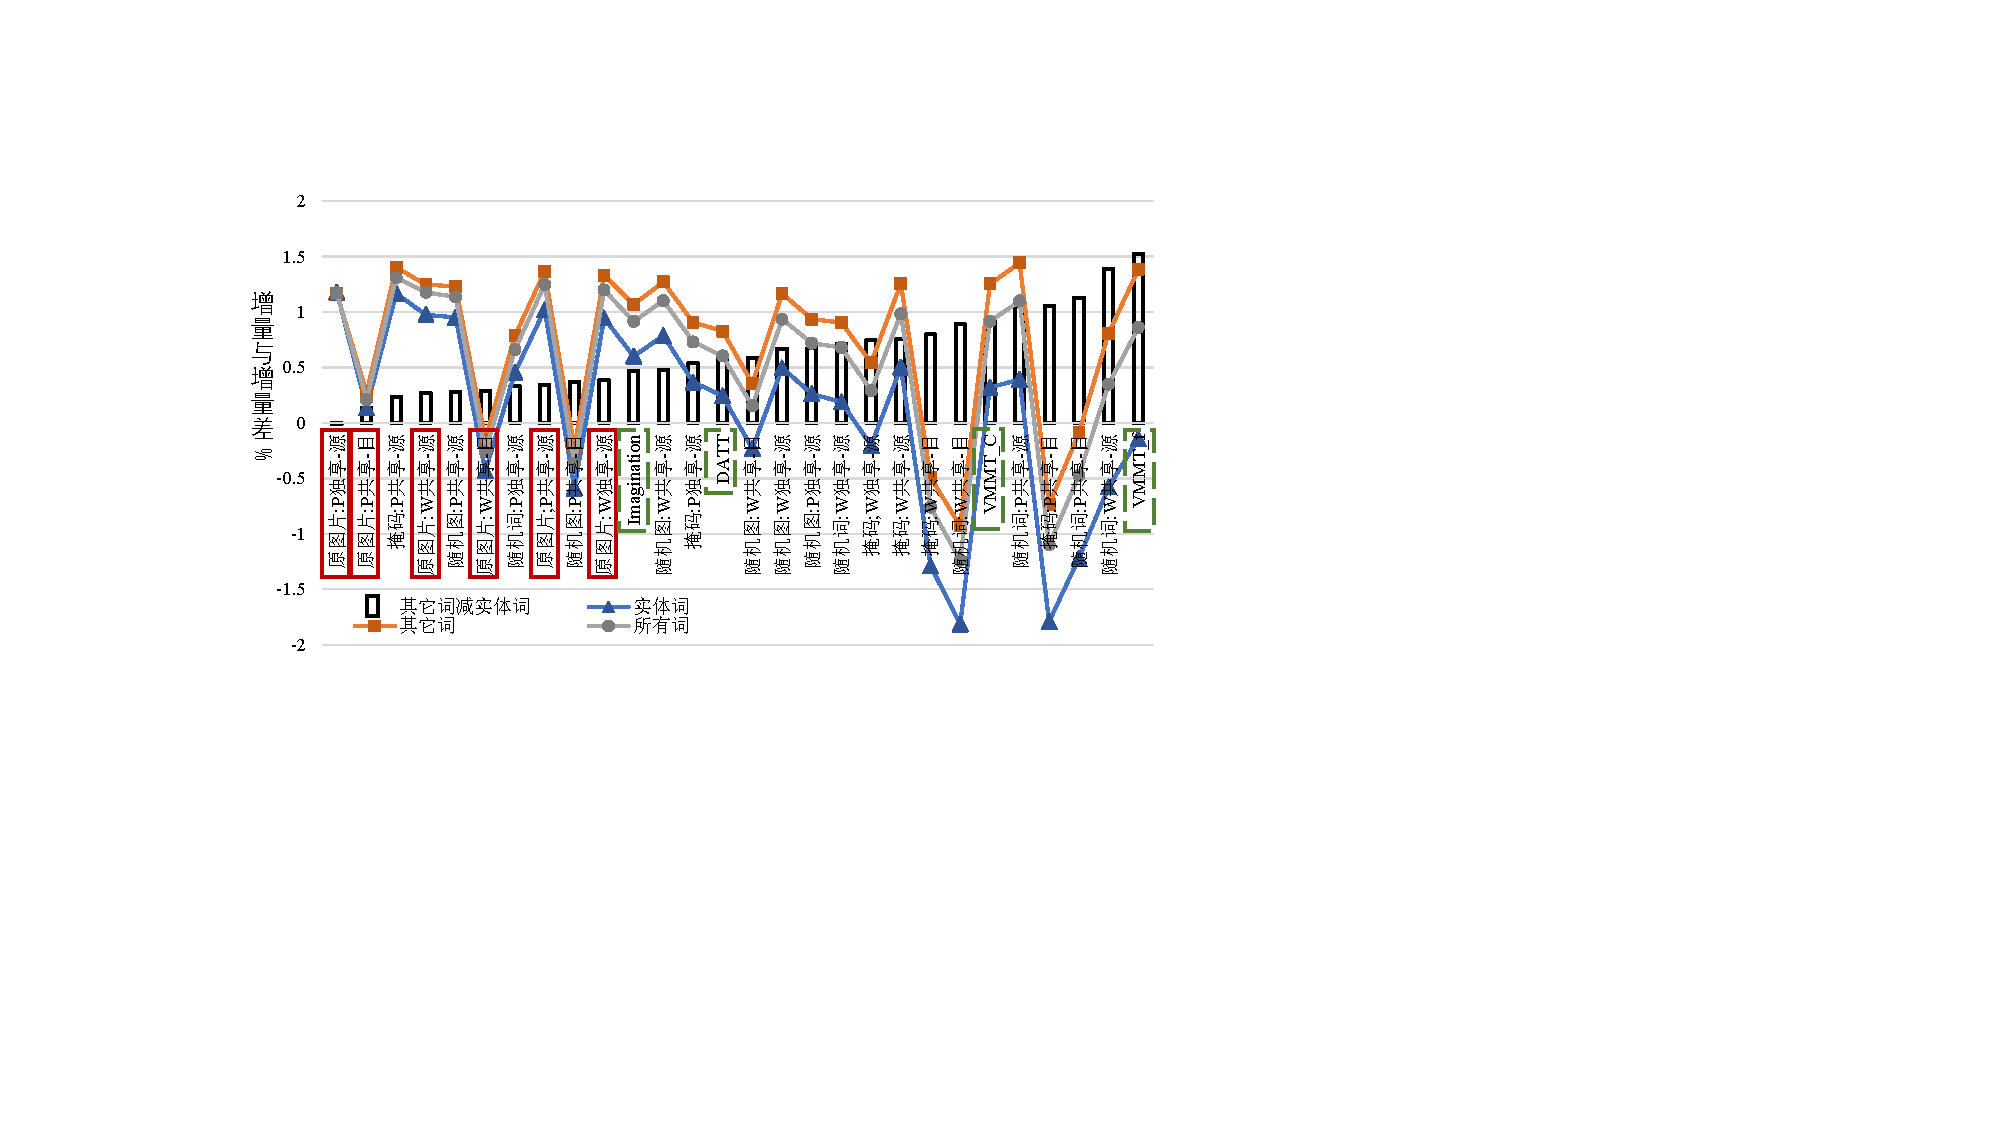
\includegraphics[scale=0.9]{Img/fig_3_analysis.pdf}
    \bicaption{实体词翻译准确率增量与增量差分析}{Accuracy increment and incremental difference analysis of entity words}
    \label{fig:3_analysis}
\end{figure}
本章选择在基于RNN的模型上进行比较。该结果需要每个方法提供模型的解码结果以及对应的纯文本基线模型的解码结果。比较的结果基于4种类型方法:6个本章的基于RNN的方法,12个\ref{sec:3_adversarial_ablation}小节中的对抗模型,6个\ref{sec:3_adversarial_ablation}小节中的掩码模型,以及4个表\ref{tab:3_rnn_ende}中的对比模型。实验结果中还展示了“所有词”的准确率,即不区分实体词或其它词的准确率。实验结果如图\ref{fig:3_analysis}所示,其中横轴代表不同的翻译系统,纵轴为增量值,蓝色线代表实体词的增量值,橘色线代表其它词的增量值,灰色线代表所有词的增量值,直方图代表其它词与实体词的增量值之差,本文称其为增量差(incremental difference)。

{\sffamily CTR-NMT:}图中实线框内的方法为本章所提CTR-NMT。图中一个值得注意的结果是,几乎所有的方法其它词的增量值都大于实体词的增量值。正如\ref{sec:3_setup_entity_extraction}小节所提到,多数实体词都是低频词,这导致模型更难学习这部分词的表示,所以当一个方法对神经翻译模型带来增益时,对所有词的提升是普遍现象,该提升也主要表现在其它词上,对实体词的提升主要依赖各类方法的特点。从图中直方图可以看到,本章所提方法的增量差普遍偏小,这说明该方法能够拉小了实体词与其它词之间增量值的差距,也就是为实体词带来的翻译准确率提升更多。

{\sffamily 对抗与消融方法:}从图中可以看出对抗评估和消融实验中使用的模型普遍得到较高增量差。仅有个别模型得到的较小的增量差。从这部分模型的整体表现可以认为降噪能力或多任务掩码方案不能够稳定提升翻译中的实体词的准确率。这进一步证明了本章所提方法能够从视觉目标中提取有价值的视觉信息。

{\sffamily 对比模型方法:}DATT、$ \mathrm{VMMT_C} $、$ \mathrm{VMMT_F} $以及Imagination并没有明显地表现出降低其它词与实体词之间增量差的能力,以上整体的对比结果表明本章所提的显式跨模态信息融合方法能够有效地主要针对实体词提升翻译准确率。

以上分析结果还表明,模型的翻译性能提升后,实体词或其它词均可以得到翻译准确率的提升。但是采用不同的方法会使这部分性能提升所侧重的方面有所差别。本章所提CTR-NMT则主要针对词实体的翻译进行优化。

\subsection{样例分析}
\begin{figure}[!htbp]
    \centering
    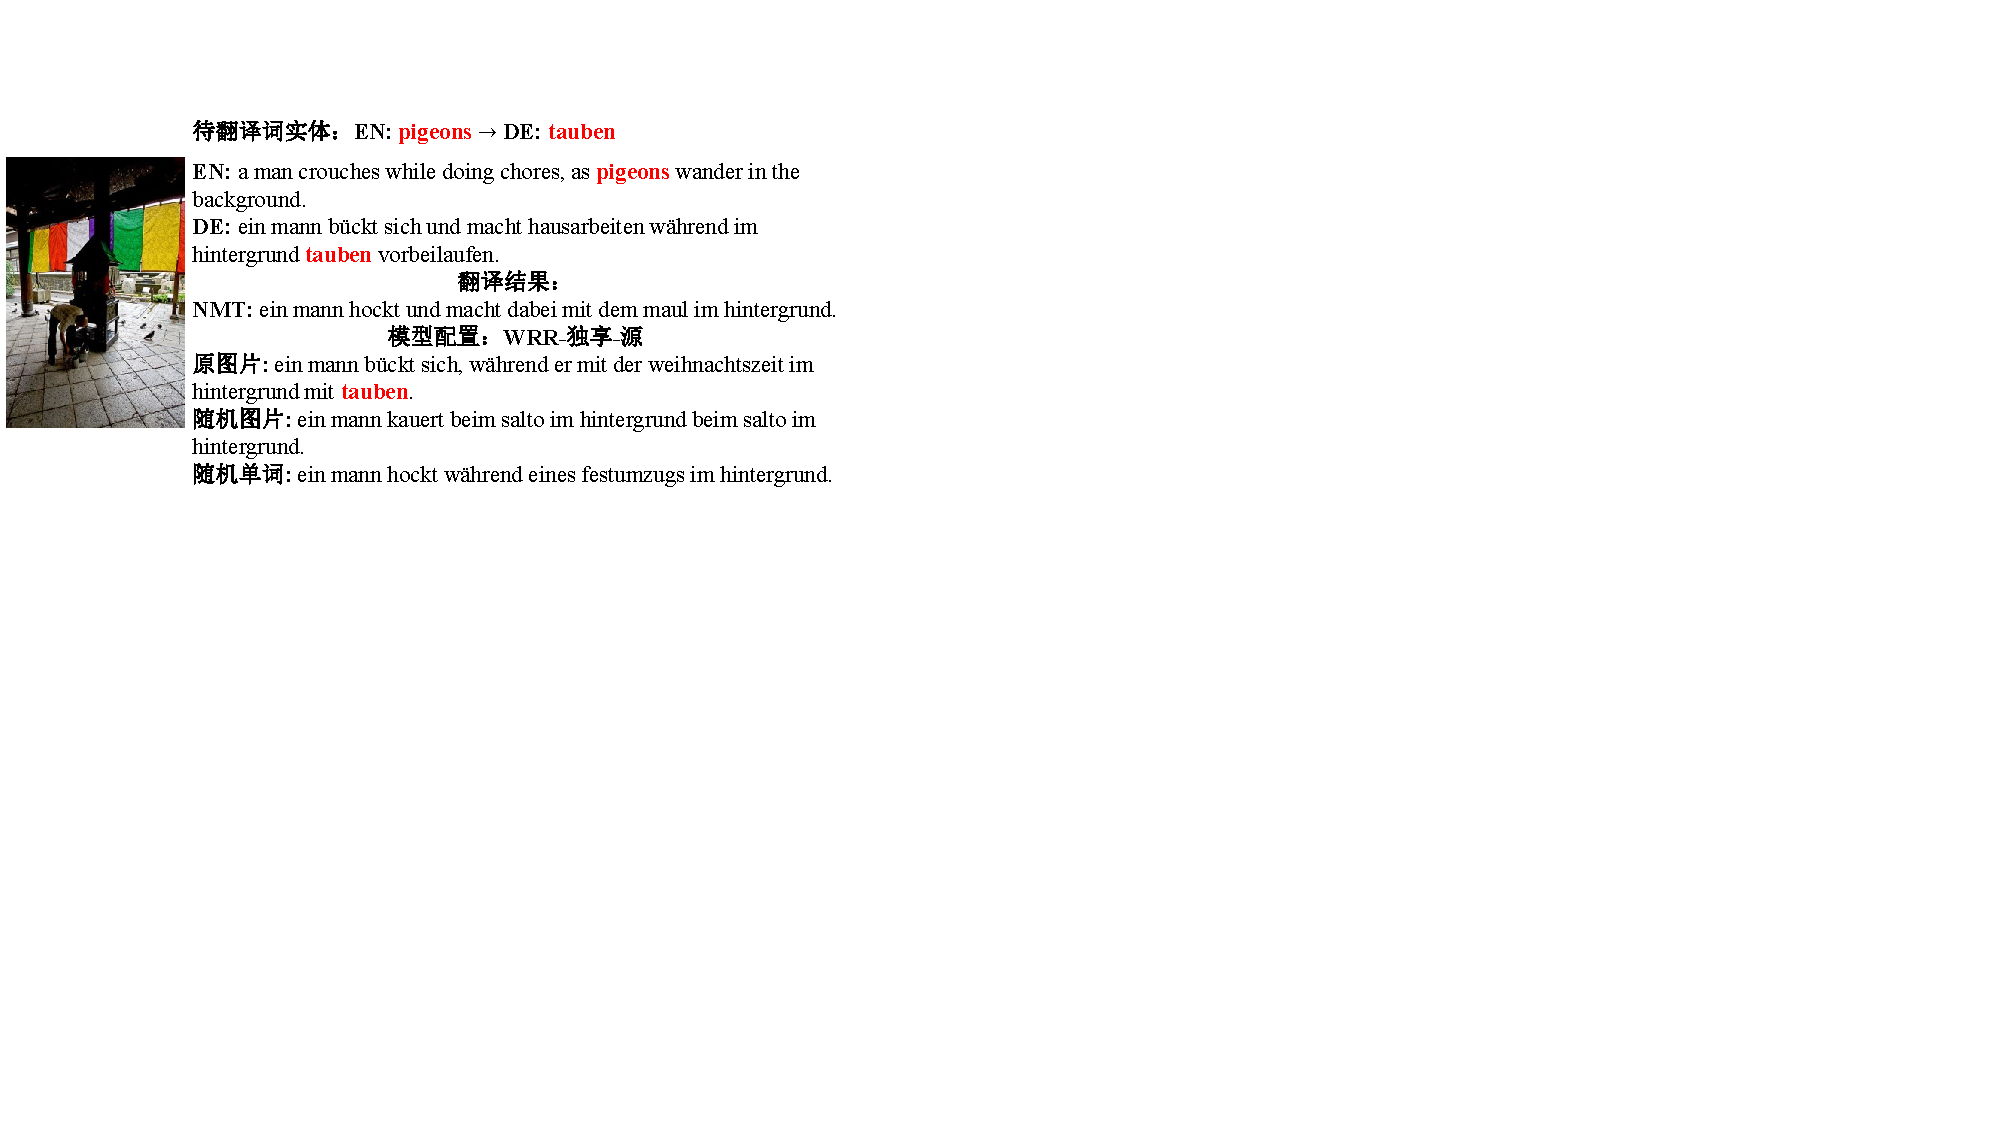
\includegraphics[scale=1.0]{Img/fig_3_case_1.pdf}
    \bicaption{实体词“pigeons”的翻译样例}{Translation example for the entity word "pigeons"}
    \label{fig:3_case_1}
\end{figure}
\begin{figure}[!htbp]
    \centering
    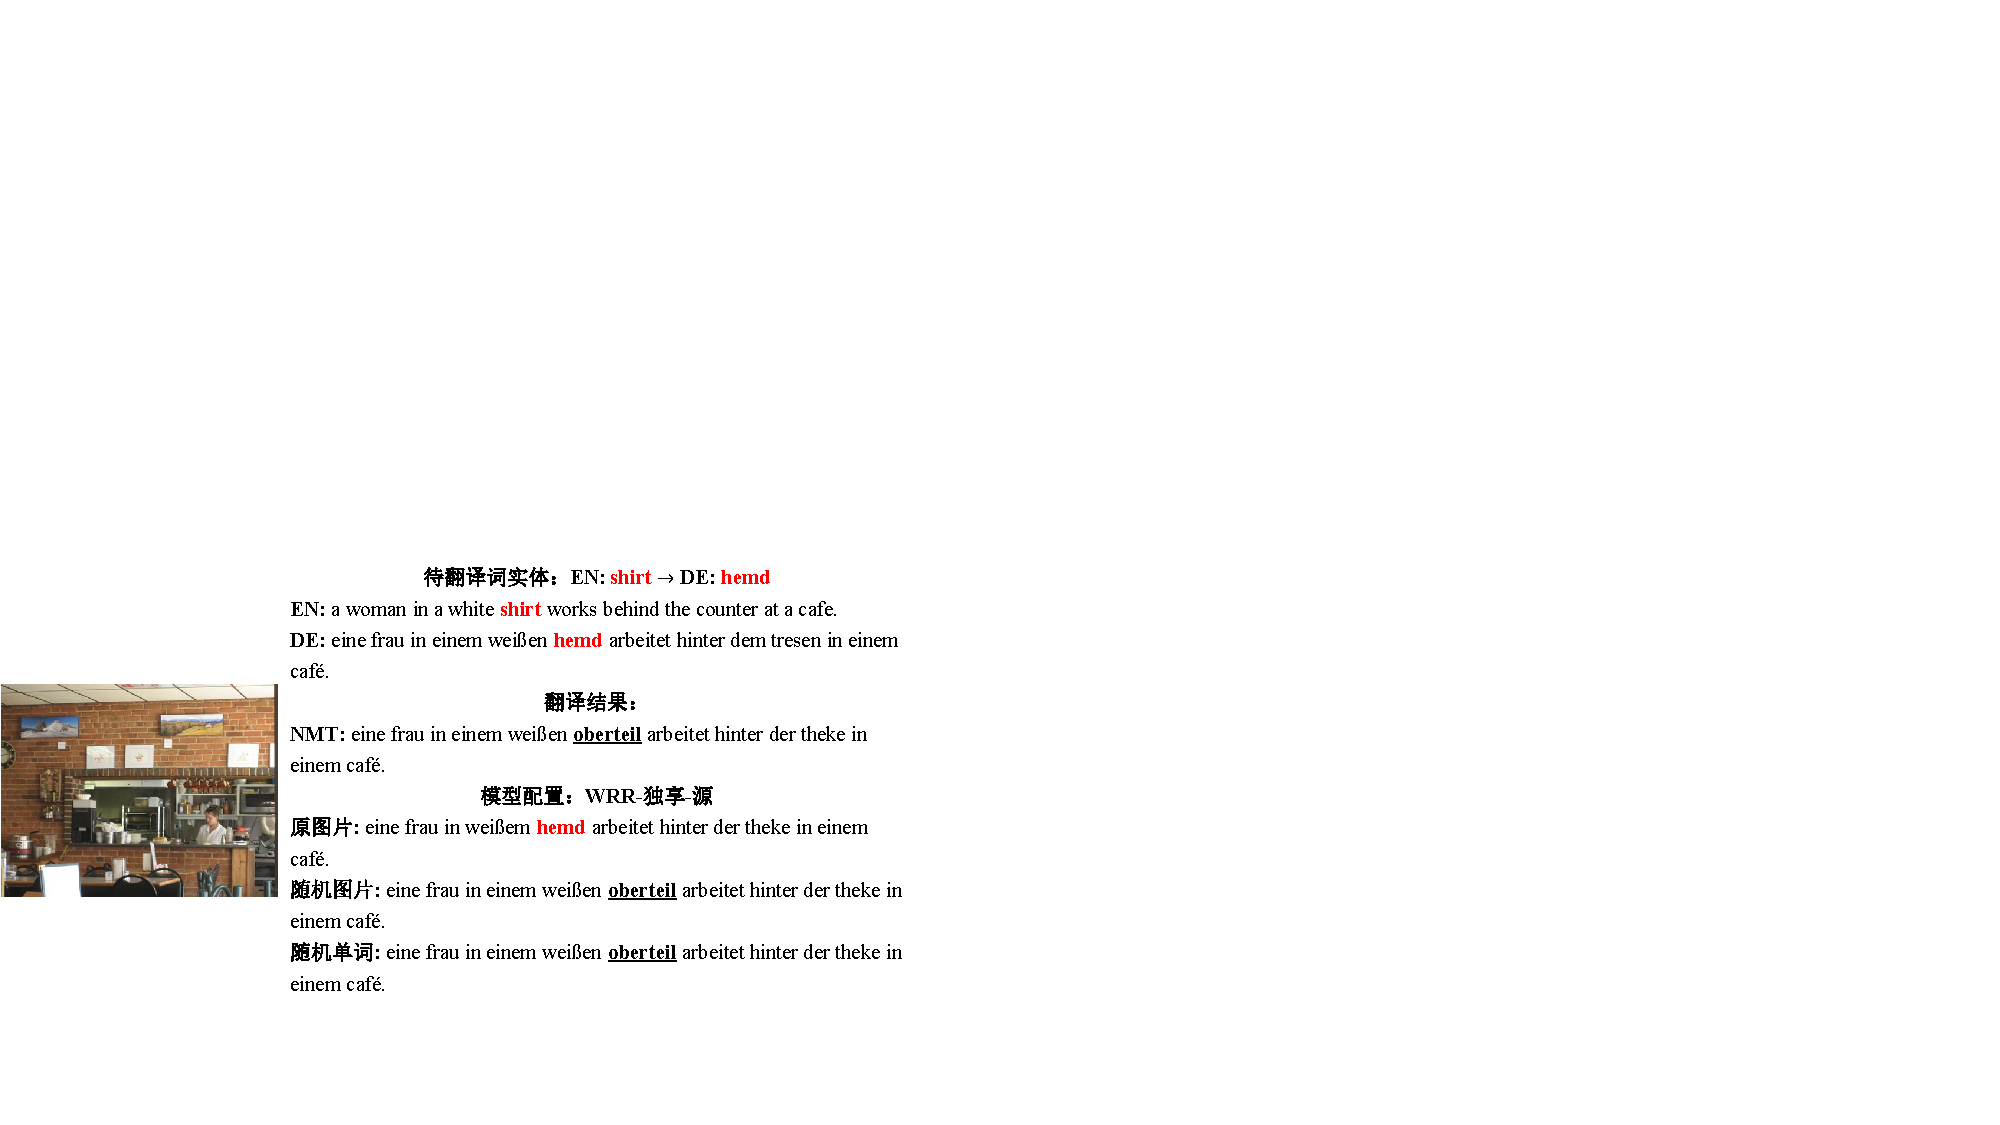
\includegraphics[scale=1.0]{Img/fig_3_case_2.pdf}
    \bicaption{实体词“shirt”的翻译样例}{Translation example for the entity word "shirt"}
    \label{fig:3_case_2}
\end{figure}
\begin{figure}[!htbp]
    \centering
    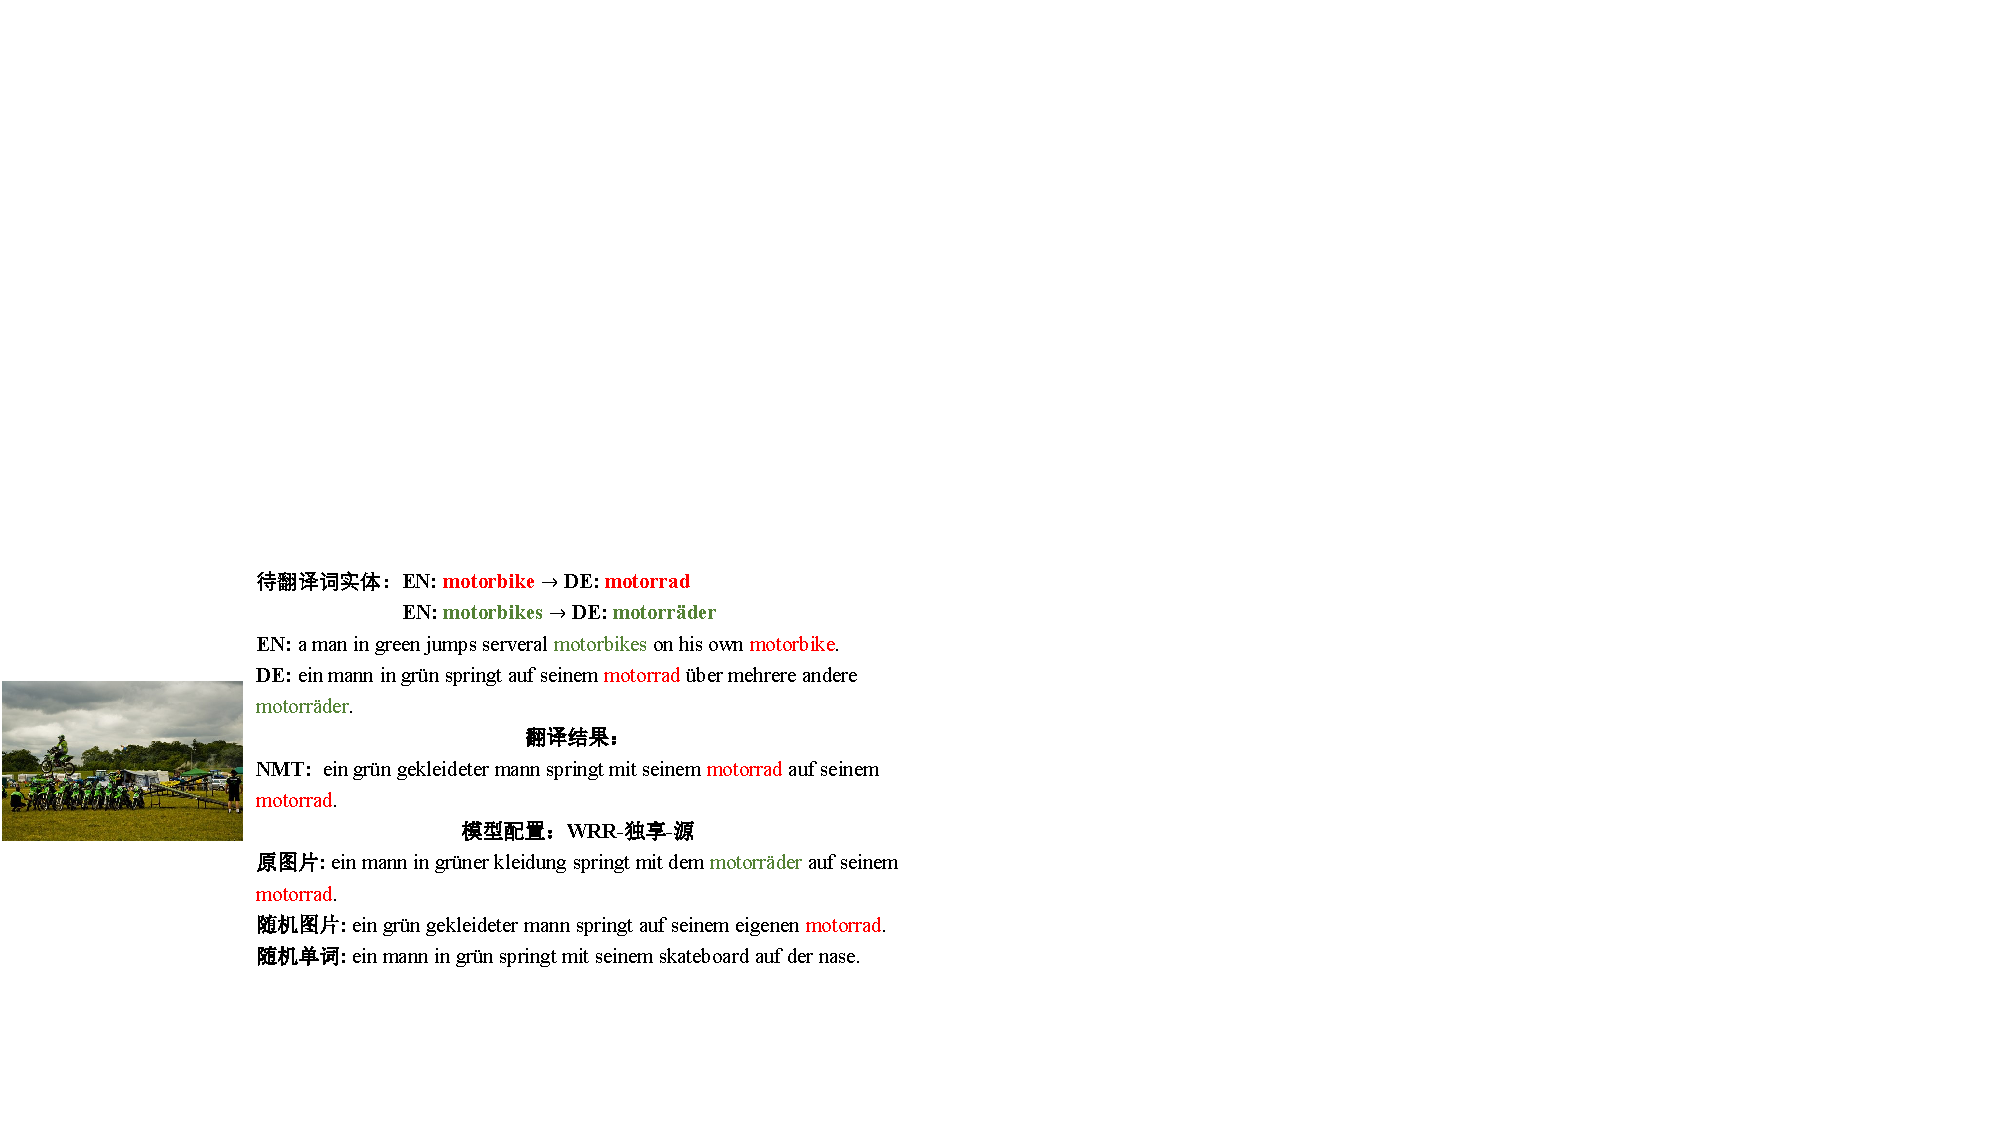
\includegraphics[scale=1.0]{Img/fig_3_case_3.pdf}
    \bicaption{实体词“motorbike”的翻译样例}{Translation example for the entity word "motorbike"}
    \label{fig:3_case_3}
\end{figure}
\begin{figure}[!htbp]
    \centering
    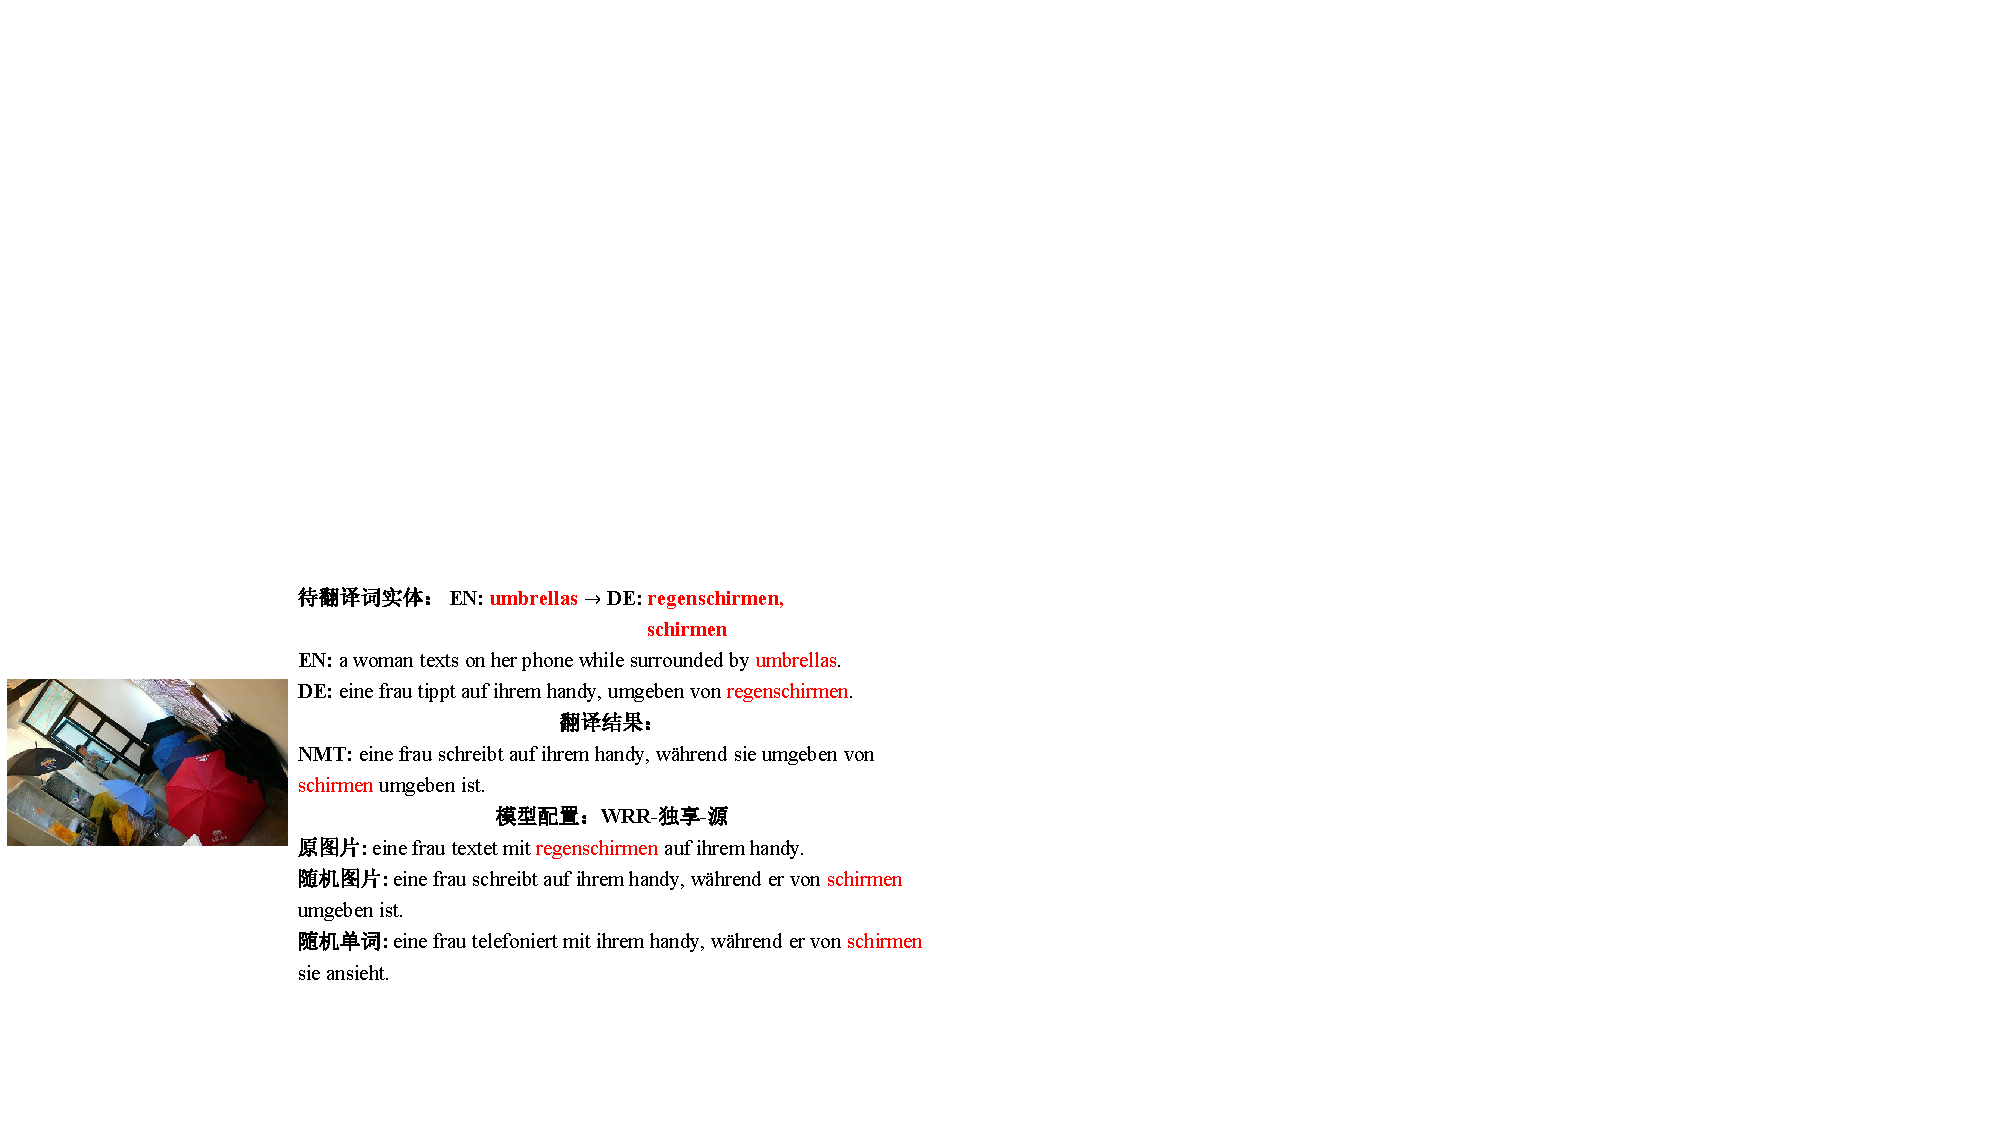
\includegraphics[scale=1.0]{Img/fig_3_case_4.pdf}
    \bicaption{实体词“umbrellas”的翻译样例}{Translation example for the entity word "umbrellas"}
    \label{fig:3_case_4}
\end{figure}

为了展示本章所提方法对句子翻译和实体词翻译带来的影响,本节在图\ref{fig:3_case_1}至\ref{fig:3_case_4}中展示了4个翻译案例。其中包含着实体词“pigeon”、“shirt”、“motorbike”和“umbrellas”的翻译。通过观察可以得到以下结论:输入正确的图片信息时,模型的性能表现相对较好;当实体词有多个译文时,其它模型的翻译结果在多个译文的表现不稳定。整体而言,本章所提方法在使用原图片时的表现更好。